% ============================================================================
%  Standalone Beamformer Architecture Diagram — VERSION 3
%  Deep saturated color-coded text with strong contrast
% ============================================================================
\documentclass[border=12pt]{standalone}
\usepackage{amsmath,amssymb}
\usepackage{tikz}
\usetikzlibrary{arrows.meta,positioning,calc,decorations.pathreplacing,fit,backgrounds}

% Define rich dark colors
\definecolor{darkblue}{RGB}{20,60,120}
\definecolor{darkred}{RGB}{140,20,20}
\definecolor{darkorange}{RGB}{160,80,0}
\definecolor{darkgreen}{RGB}{0,90,40}
\definecolor{darkpurple}{RGB}{80,20,110}
\definecolor{darkgray}{RGB}{50,50,50}
\definecolor{annotgray}{RGB}{40,40,40}

\begin{document}
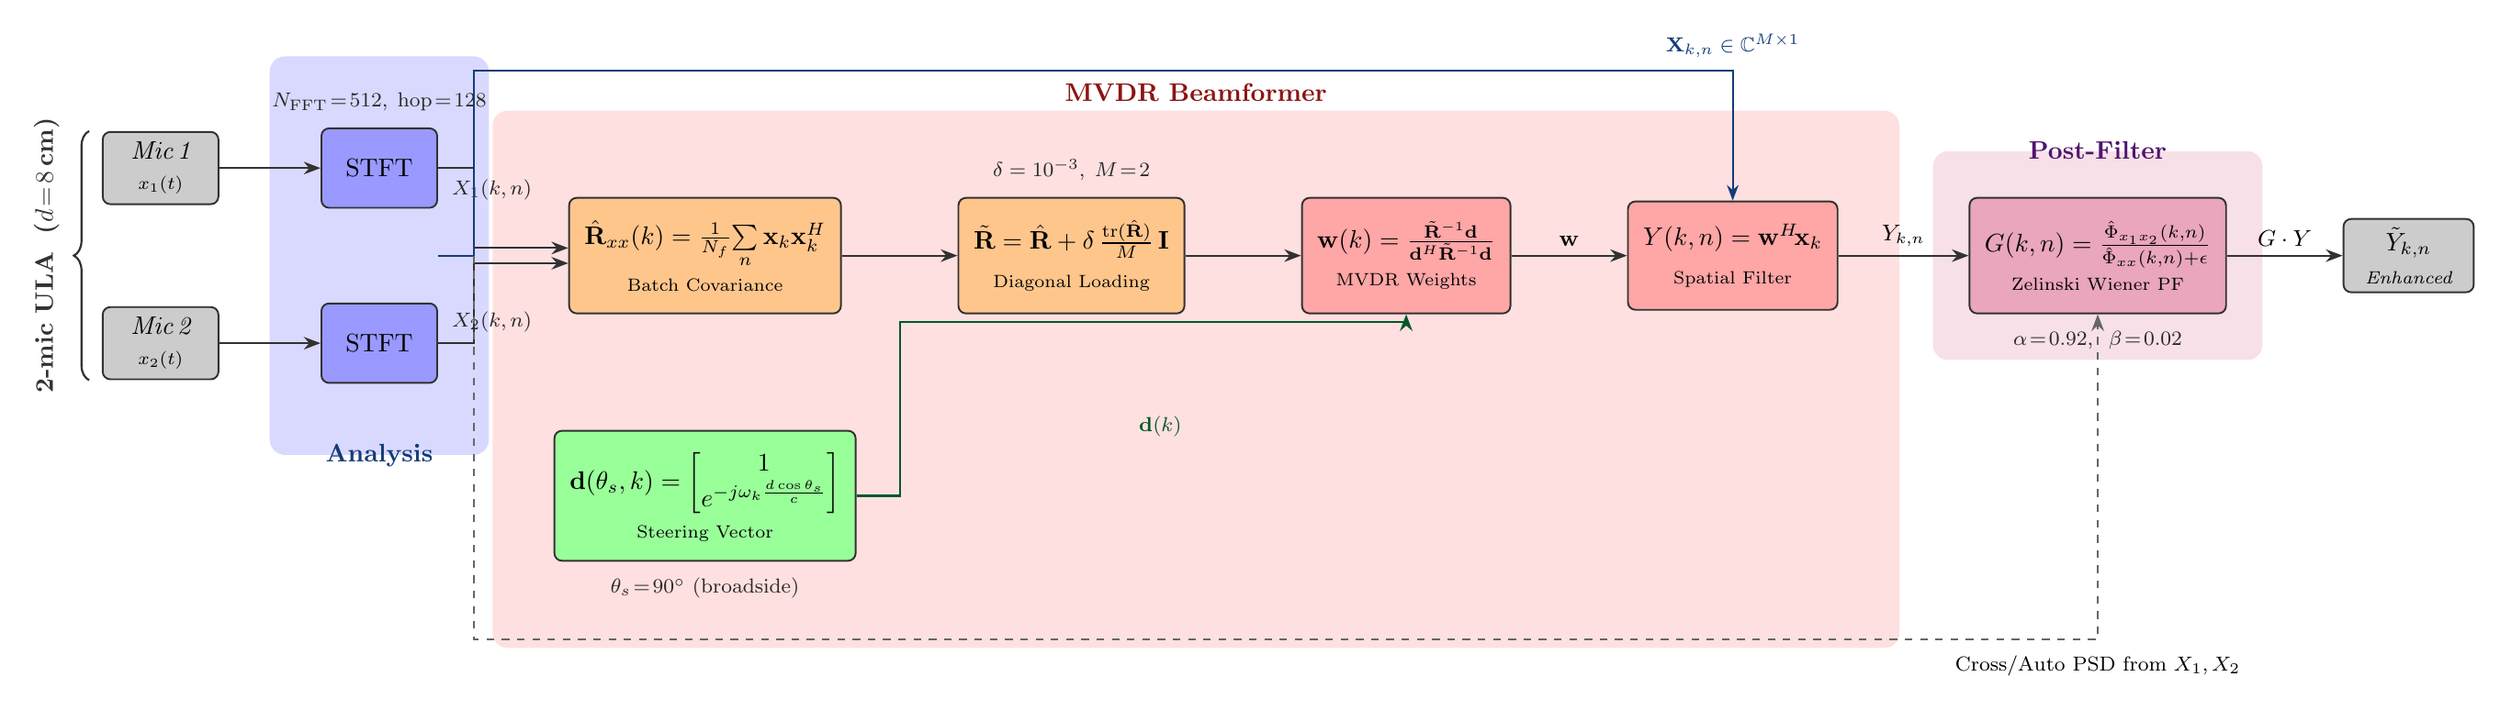
\begin{tikzpicture}[
    >=Stealth,
    node distance=1.2cm and 1.0cm,
    block/.style={draw=darkgray, rounded corners=3pt, minimum height=1.1cm,
                  minimum width=2.0cm, align=center, font=\normalsize,
                  fill=#1, text=black, line width=0.7pt,
                  inner xsep=6pt, inner ysep=6pt},
    block/.default=white,
    io/.style={draw=darkgray, rounded corners=3pt, minimum height=1.0cm,
               minimum width=1.6cm, align=center, font=\normalsize\itshape,
               fill=gray!40, text=black, line width=0.7pt},
    arr/.style={->, thick, line width=0.8pt, darkgray},
    darr/.style={->, thick, dashed, black!60, line width=0.8pt},
    lbl/.style={font=\small, midway, text=black},
    stagelbl/.style={font=\small\bfseries},
    annot/.style={font=\footnotesize, text=annotgray},
  ]

  % ===== MICROPHONES =====
  \node[io] (mic1) {Mic\,1\\ \scriptsize $x_1(t)$};
  \node[io, below=1.4cm of mic1] (mic2) {Mic\,2\\ \scriptsize $x_2(t)$};

  % ULA brace
  \draw[decorate, decoration={brace, amplitude=6pt, mirror},
        thick, darkgray]
    ([xshift=-5pt]mic1.north west) -- ([xshift=-5pt]mic2.south west)
    node[midway, left=8pt, rotate=90, anchor=south,
         font=\normalsize\bfseries, text=darkgray] {2-mic ULA\; ($d\!=\!8$\,cm)};

  % ===== STFT =====
  \node[block=blue!40, right=1.4cm of mic1, minimum width=1.6cm] (stft1)
       {STFT};
  \node[block=blue!40, right=1.4cm of mic2, minimum width=1.6cm] (stft2)
       {STFT};

  \draw[arr] (mic1) -- (stft1);
  \draw[arr] (mic2) -- (stft2);

  % STFT annotation
  \node[annot, above=3pt of stft1]
       {$N_\text{FFT}\!=\!512,\; \text{hop}\!=\!128$};
  \node[annot, right=2pt of stft1.south east, anchor=south west]
       {$X_1(k,n)$};
  \node[annot, right=2pt of stft2.north east, anchor=north west]
       {$X_2(k,n)$};

  % ===== COVARIANCE ESTIMATION =====
  \node[block=orange!45, right=1.8cm of $(stft1.east)!0.5!(stft2.east)$,
        minimum width=2.6cm, minimum height=1.6cm] (cov)
       {$\hat{\mathbf{R}}_{xx}(k) = \frac{1}{N_f}\!\sum\limits_n
         \mathbf{x}_k\mathbf{x}_k^H$\\[3pt]
        {\scriptsize Batch Covariance}};

  % Lines from STFT to Cov
  \draw[arr] (stft1.east) -- ++(0.5,0) |- ([yshift=3pt]cov.west);
  \draw[arr] (stft2.east) -- ++(0.5,0) |- ([yshift=-3pt]cov.west);

  % ===== STEERING VECTOR =====
  \node[block=green!40, below=1.6cm of cov,
        minimum width=2.6cm, minimum height=1.8cm] (steer)
       {$\mathbf{d}(\theta_s,k) = \begin{bmatrix}1\\
         e^{-j\omega_k\frac{d\cos\theta_s}{c}}\end{bmatrix}$\\[3pt]
        {\scriptsize Steering Vector}};

  % Angle annotation
  \node[annot, below=3pt of steer]
       {$\theta_s\!=\!90^\circ$ (broadside)};

  % ===== DIAGONAL LOADING =====
  \node[block=orange!45, right=1.6cm of cov,
        minimum width=2.6cm, minimum height=1.6cm] (diag)
       {$\tilde{\mathbf{R}} = \hat{\mathbf{R}}
         + \delta\,\frac{\mathrm{tr}(\hat{\mathbf{R}})}{M}\,\mathbf{I}$\\[3pt]
        {\scriptsize Diagonal Loading}};

  \draw[arr] (cov) -- node[lbl, above] {} (diag);
  \node[annot, above=3pt of diag] {$\delta=10^{-3},\; M\!=\!2$};

  % ===== MVDR WEIGHTS =====
  \node[block=red!35, right=1.6cm of diag,
        minimum width=2.6cm, minimum height=1.6cm] (mvdr)
       {$\mathbf{w}(k) =
         \frac{\tilde{\mathbf{R}}^{-1}\mathbf{d}}
              {\mathbf{d}^H\tilde{\mathbf{R}}^{-1}\mathbf{d}}$\\[3pt]
        {\scriptsize MVDR Weights}};

  \draw[arr] (diag) -- (mvdr);

  % Steering vector to MVDR
  \draw[arr, darkgreen]
    (steer.east) -- ++(0.6,0) |- ([yshift=-3pt]mvdr.south) -- (mvdr.south);
  \node[annot, text=darkgreen] at ($(steer.east)!0.5!(mvdr.south)+(0.4,-0.3)$)
       {$\mathbf{d}(k)$};

  % ===== BEAMFORM (apply weights) =====
  \node[block=red!35, right=1.6cm of mvdr,
        minimum width=2.4cm, minimum height=1.5cm] (apply)
       {$Y(k,n)=\mathbf{w}^H\!\mathbf{x}_k$\\[3pt]
        {\scriptsize Spatial Filter}};

  \draw[arr] (mvdr) -- node[lbl, above] {$\mathbf{w}$} (apply);

  % Feed STFT data to beamform (long path on top)
  \coordinate (stftmid) at ($(stft1.east)!0.5!(stft2.east)$);
  \draw[arr, darkblue, line width=0.7pt]
    (stftmid) -- ++(0.5,0) coordinate (junc)
    |- ([yshift=1.8cm]apply.north) -- (apply.north);
  \node[annot, text=darkblue, above=1.85cm of apply]
       {$\mathbf{X}_{k,n}\in\mathbb{C}^{M\times 1}$};

  % ===== ZELINSKI POST-FILTER =====
  \node[block=purple!35, right=1.8cm of apply,
        minimum width=2.8cm, minimum height=1.6cm] (pf)
       {$G(k,n) =
         \frac{\hat{\Phi}_{x_1 x_2}(k,n)}
              {\hat{\Phi}_{xx}(k,n)+\epsilon}$\\[3pt]
        {\scriptsize Zelinski Wiener PF}};

  \draw[arr] (apply) -- node[lbl, above] {$Y_{k,n}$} (pf);

  % PF parameters annotation
  \node[annot, below=3pt of pf]
       {$\alpha\!=\!0.92,\;\; \beta\!=\!0.02$};

  % Cross-PSD input from STFT (dashed, bottom path)
  \draw[darr]
    (junc) |- ([yshift=-4.5cm]pf.south) -- (pf.south);
  \node[annot, text=black, below=4.6cm of pf, anchor=north]
       {Cross/Auto PSD from $X_1,X_2$};

  % ===== OUTPUT =====
  \node[io, right=1.6cm of pf, minimum width=1.8cm] (out)
       {$\tilde{Y}_{k,n}$\\[1pt]\scriptsize Enhanced};
  \draw[arr] (pf) -- node[lbl, above] {$G \cdot Y$} (out);

  % ===== STAGE LABELS (background regions) =====
  \begin{scope}[on background layer]
    % STFT stage
    \node[fill=blue!15, rounded corners=6pt,
          fit=(stft1)(stft2),
          inner xsep=20pt, inner ysep=28pt] (stftbox) {};
    \node[stagelbl, text=darkblue, font=\normalsize\bfseries] at (stftbox.south)
         {Analysis};

    % MVDR stage
    \node[fill=red!12, rounded corners=6pt,
          fit=(cov)(diag)(mvdr)(apply)(steer),
          inner xsep=24pt, inner ysep=34pt] (mvdrbox) {};
    \node[stagelbl, text=darkred, font=\normalsize\bfseries,
          anchor=south] at (mvdrbox.north)
         {MVDR Beamformer};

    % Post-filter stage
    \node[fill=purple!12, rounded corners=6pt,
          fit=(pf),
          inner xsep=14pt, inner ysep=18pt] (pfbox) {};
    \node[stagelbl, text=darkpurple, font=\normalsize\bfseries] at (pfbox.north)
         {Post-Filter};
  \end{scope}

\end{tikzpicture}
\end{document}
